\chapter{Companies and Financial Accounting}
\section{Companies}
\subsection{What is a company?}
A company is a legal entity (``personality'') that can issue contracts, enter into agreements or contracts, assume obligations, incur and pay debts, sue and be sued in its own right, and be held responsible for its own actions. There are three main types of companies in the UK:
\begin{enumerate}
    \item A Sole Trader
    \item A Partnership
    \item A Limited Liability Company
\end{enumerate}
\subsubsection{Sole Trader}
A sole Trader:
\begin{itemize}
    \item Runs their own business as an individual
    \item Keeps all of the net profits
    \item Is personally responsible for any losses their business makes (unlimited liability)
\end{itemize}
\subsubsection{Partnership}
A Partnership:
\begin{itemize}
    \item Involves two or more partners who share responsibility for the business
    \item Keeps all of the net profits (jointly)
    \item Is jointly responsible for any losses their business makes (joint unlimited liability)
    \item A partner does not have to be an actual person. For example, a limited company counts as a `legal person' and can also be a partner
\end{itemize}
\subsubsection{Limited Liability Company}
A Limited Liability Company that is ``limited by shares'' or ``limited by guarantee.''

Limited by shares:
\begin{itemize}
    \item Usually businesses that make a profit
          \begin{itemize}
              \item is legally separate from those who run it (limited liability)
              \item has shares and shareholders
              \item retains net profits
          \end{itemize}
\end{itemize}

Limited by guarantee:
\begin{itemize}
    \item Usually businesses that are ``not for profit''
          \begin{itemize}
              \item is legally separate from those who run it (limited liability)
              \item has guarantors and a ``guaranteed amount''
              \item invests profits it makes back into the company
          \end{itemize}
\end{itemize}
\subsection{Structure of a Limited Liability Company limited by shares}
\begin{figure}[H]
    \centering
    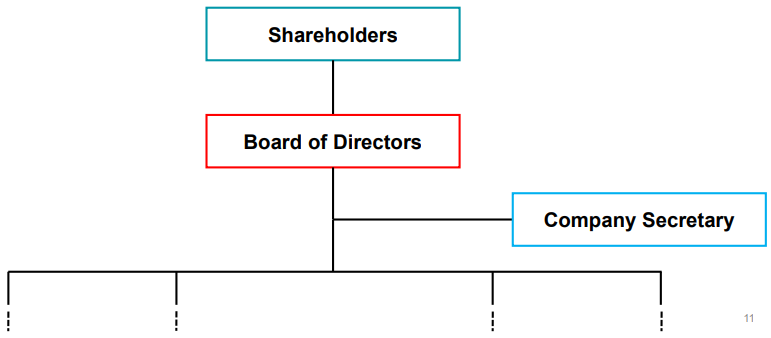
\includegraphics[width = \textwidth]{./img/figure26.png}
    \caption{Structure of a Limited Liability Company limited by shares.}
\end{figure}
\subsection{What is a shareholder?}
\begin{itemize}
    \item Shareholders own a Limited Liability Company limited by shares
    \item They have no day-to-day duties related to the company's operation
    \item Each shareholder owns a fraction of the company (and has corresponding voting power) proportional to their shareholding (investment)
    \item The liability of shareholders is limited to their original investment
    \item The company's profits are paid to shareholders as share dividend
\end{itemize}
\subsection{What is the Board of Directors?}
\begin{itemize}
    \item The Board of Directors is elected by the shareholders at the Annual General Meeting (AGM) to run the company.
          \begin{itemize}
              \item Directors may also be shareholders (but not necessarily)
              \item The shareholders can vote to appoint or sack individual Board of Directors members
          \end{itemize}
    \item The Board of Directors files the company's audited accounts (legal requirement)
    \item The Board of Directors report to the shareholders at the AGM (legal requirement)
    \item The Board of Directors is controller by the Chairman of the Board
    \item The Board of Directors can appoint or sack the Chief Executive Officer (CEO - responsible for day-to-day running)
\end{itemize}
\subsection{What is a company secretary?}
The company secretary ensures the smooth administration of the company. The company secretary is responsible for:
\begin{itemize}
    \item Making sure the company stays within the law
    \item Making sure the company maintains proper record books and accounts
    \item Providing strategic advice to the Board of Directors (sometimes)
\end{itemize}
The company secretary may or may not be a member of the Board of Directors.
\subsection{Limited Liability Company}
A Limited Liability Company that is ``limited by shares'' can be public or private.

Private Limited Company (Ltd.):
\begin{itemize}
    \item Share ownership is controlled
          \begin{itemize}
              \item is owned privately
              \item only one director is required
              \item have nine months to file their annual accounts
              \item a company secretary is not legally required
          \end{itemize}
\end{itemize}

Public Limited Company (PLC):
\begin{itemize}
    \item Share ownership is NOT controlled
          \begin{itemize}
              \item company shares can be bought and sold publically on the open market (a stock exchange)
              \item two directors are required
              \item have six months to file their annual accounts
              \item a company secretary is legally required
          \end{itemize}
\end{itemize}
\section{What is accounting?}
Accounting is the collection, analysis and communication of financial information that is used by:
\begin{itemize}
    \item Those who need to make decisions and plans in an organisation
    \item Those who need to control an organisation
\end{itemize}
Accounting helps companies to plan for the future and evaluate past performance. Accounting os often referred to as the language of business.
\section{The fundamental accounting equation}
\begin{gather}
    \textrm{Assets} = \textrm{Liabilities} + \textrm{Owners' Equity}
\end{gather}
where:
\begin{itemize}
    \item Assets are resources that a company owns. They have the capacity to provide future services or benefits. Companies use their assets in carrying out activities like production and sales
    \item Liabilities are claims against assets - existing debts and obligations. They arise from purchasing items on credit or borrowing money from a bank for purchases
    \item Owners' Equity is what remains of the assets after all liabilities have been paid
\end{itemize}
``Liabilities + Owners' Equity'' are the rights or claims against the resources of the company.
\begin{table}[H]
    \centering
    \begin{tabular}{@{}lll@{}}
        \toprule
        \textbf{Assets} & \textbf{Liabilities} & \textbf{Owners' Equity}\\
        \midrule
        Cash & Wages due & Owners' capital\\
        Equipment & Bank debt &\\
        Buildings & Accounts payable &\\
        Land & & \\
        Inventories & & \\
        \bottomrule
    \end{tabular}  
    \caption{Table to show Assets, Liabilities and Owners' Equity.}  
\end{table}
\subsection{Some important definitions}
\textbf{Assets:}
\begin{quoting}
    Economic resources that a company expects to help generate future cash inflows or help reduce future cash outflow.
\end{quoting}
\textbf{Current assets:}
\begin{quoting}
    A company's cash and other assets that are expected to be converted to cash over the next one year period.
\end{quoting}
\textbf{Non-current assets:}
\begin{quoting}
    A company's assets that are not expected to be converted to cash over the next one year period.
\end{quoting}
\textbf{Inventory:}
\begin{quoting}
    Goods (current assets) available for sale or raw materials and components used to produce goods available for sale.
\end{quoting}
\textbf{Liabilities:}
\begin{quoting}
    Economic obligations of the organisation to outsiders, or claims against its assets by outsiders.
\end{quoting}
\textbf{Current liabilities:}
\begin{quoting}
    A company's short term obligations, due within one year period.
\end{quoting}
\textbf{Non-current liabilities:}
\begin{quoting}
    A company's long-term obligations listed on the balance sheet.
\end{quoting}
\textbf{Dividends:}
\begin{quoting}
    Money paid regularly to shareholders by the company.
\end{quoting}
\section{Balance sheet}
The balance sheet is one of the two most common accounting statements. The fundamental accounting equation defines the format of the balance sheet. The balance sheet shows the financial position of the company at one instant in time (e.g. end of the quarter or end of the year).
\begin{table}[H]
    \centering
    \begin{tabular}{@{}llll@{}}
        \toprule
        Assets              &               & Liabilities / Owners' Equity &               \\
        \midrule
        Cash                & \pounds 2,500 & Accounts payable             & \pounds 1,200 \\
        Land                & \pounds 1,800 & Bank note                    & \pounds 900   \\
        Accounts receivable & \pounds 800   & Owners' Equity               & \pounds 3,000 \\
        \midrule
        Total assets        & \pounds 5,100 & Total liabilities and        & \pounds 5,100 \\
                            &               & Owners' Equity               &               \\
        \bottomrule
    \end{tabular}
    \caption{Balance sheet.}
\end{table}
\begin{gather}
    \textrm{Assets} = \textrm{Liabilities} + \textrm{Owners' Equity} = \pounds 5100
\end{gather}
\section{Income statement}
The income statement is the second of the two most common accounting statements. The income statement summarises the revenue and expense results of operations over a period of time (a moving picture.) It is defined by the following equation:
\begin{gather}
    \textrm{Profit (or Loss)} = \textrm{Revenues} - \textrm{Expenses}
\end{gather}
\begin{table}[H]
    \centering
    \begin{tabular}{@{}llll@{}}
        \toprule
        \textbf{Revenue}    &                &               &               \\
        Sales               &                &               & \pounds 3,000 \\
        \midrule
        \textbf{Expenses}   &                &               &               \\
        Labour              &                & \pounds 1,200 &               \\
        Depreciation        &                & \pounds 400   &               \\
        Material            &                & \pounds 500   &               \\
        \midrule
                            & Total Expenses &               & \pounds 2,100 \\
        \textbf{Net income} &                &               & \pounds 900   \\
        \bottomrule
    \end{tabular}
    \caption{Income statement.}
\end{table}
\subsection{Some important definitions}
\textbf{Turnover:}
\begin{quoting}
    The net sales generated by a business.
\end{quoting}
Turnover and profit are the beginning and end points of the income statement.
\section{Worked example}
John Deere owns and operates a design company called Deere Consulting Ltd. The financial position of his business is:
\begin{table}[H]
    \centering
    \begin{tabular}[]{@{}ll@{}}
        \toprule
        Cash                & \pounds 1,720  \\
        Accounts receivable & \pounds 3,240  \\
        Land                & \pounds 24,100 \\
        Accounts payable    & \pounds 5,400  \\
        John Deere, Capital & \pounds 23,660 \\
        \bottomrule
    \end{tabular}
    \caption{Financial position of John Deere Ltd.}
\end{table}
During May 2021, the following events occurred:
\begin{enumerate}
    \item Deere received \pounds 12,000 as a gift and deposited the cash in the business bank account
    \item Deere paid of the beginning balance of the accounts payable
    \item Deere performed services for a client and received cash of \pounds 1,100
    \item Deere collected \pounds 750 cash from a customer on account
    \item Deere purchased \pounds 720 of supplies on account
    \item Deere billed a client \pounds 5,000 for services rendered
    \item Deere invested personal cash of \pounds 1,700 in the business
    \item Deere recorded \pounds 1,860 of business expenses
    \item Deere sold supplies to another company for \pounds 80 cash (the price of the supplies)
    \item Deere withdrew \pounds 4,000 cash for personal use
\end{enumerate}
For Deere Consulting Ltd., prepare:
\begin{enumerate}
    \item The income statement for the month ended 31 May 2021
    \item The balance sheet as at 31 May 2021
\end{enumerate}
\subsubsection{Income statement, month ended 31 May, 2021}
\begin{table}[H]
    \centering
    \begin{tabular}{@{}llll@{}}
        \toprule
        \textbf{Revenue} & & & \\
        & Services to Client 1 & \pounds 5,000 & \\
        & Services to Client 2 & \pounds 1,100 & \\
        & Total revenue & & \pounds 6,100 \\
        \midrule
        \textbf{Expenses} & & & \\
        & Business expenses & & \pounds 1,860 \\
        \midrule
        \textbf{Net income} & & & \pounds 4,240 \\
        \bottomrule
    \end{tabular}
    \caption{Deere Consulting Ltd. income statement, month ended 31 May, 2021.}
\end{table}
\subsubsection{Balance sheet, 31 May, 2021}
\begin{table}[H]
    \centering
    \begin{tabular}{@{}llll@{}}
        \toprule
        \textbf{Assets} & & \textbf{Liabilities/Owners' Equity}\\
        \midrule
        Cash & \pounds 6,090 & Accounts payable & \pounds 720\\
        Accounts receivable & \pounds 7,490 & & \\
        Supplies & \pounds 640 & & \\
        Land & \pounds 24,100 & J. Deere, Capital & \pounds 37,600 \\
        \midrule
        \textbf{Total assets} & \pounds 38,320 & \textbf{Total liabilities and} & \pounds 38,320\\
        & & \textbf{Owners' Equity} & \\
        \bottomrule
    \end{tabular}
\end{table}
\section{Cash flow statement}
The cash flow statement shows how a ompany generated the cash flows it needed to finance its various opportunities and responsibilities over a period of time (a moving picture). It acts as a bridge between the income statement and the balance sheet by showing how money moved in and out of the business. The cash flow statement has three primary sections:
\begin{enumerate}
    \item Cash flow from operating activities
    \begin{itemize}
        \item Cash inflows: generation of funds in normal operations
        \item Cash outflows: expenduture of funds in normal operations
    \end{itemize}
    \item Cash flow from investing activities
    \begin{itemize}
        \item Cash inflows: sale of plant and equipment. Liquidation of long-term investment
        \item Cash outflows: purchase of plant and equipment. Long-term investments
    \end{itemize}
    \item Cash flow from financing activities
    \begin{itemize}
        \item Cash inflows: sale of bonds, common stock and other securities
        \item Csh outflows: repurchase of bonds, common stock and other securities. Payment of cash dividend
    \end{itemize}
\end{enumerate}
The sum of these sections = net cash flow.
\subsection{Cash flow statement}
\begin{table}[H]
    \centering
    \begin{tabular}{@{}ll@{}}
        \toprule
        \textbf{Cash flows from operating activities} & \\
        Cash generated from operations & \pounds 5,460\\
        Income tax paid & -\pounds 1,351\\
        Interest paid & -\pounds 40\\
        \midrule
        Net cash flow from operating activities & \pounds 4,069\\
        \midrule
        \textbf{Cash flows from investing activities} & \\
        Interest received & \pounds 100\\
        Purchases of property, plant and equipment & \pounds 5,894\\
        Proceeds on disposal of property & \pounds 41\\
        Capital grants received & \pounds 1,979\\
        \midrule
        Net cash flow from investing activities & -\pounds 3,774\\
        \midrule
        \textbf{Cash flows from financing activities} & \\
        Repayments of borrowings & -\pounds 10,991\\
        New loans raised & \pounds 10,841\\
        Repayment of liase liabilities & -\pounds 107\\
        \midrule
        Net cash flow from financing activities & -\pounds 257\\
        \midrule
        Net increase/(decrease) in cash and cash equivalents & \pounds 38\\
        Cash and cash equivalents at beginning of the period & \pounds 430\\
        \midrule
        \textbf{Cash and cash equivalents at end of year} & \pounds 522\\
        \bottomrule
    \end{tabular}
    \caption{Cash flow statement.}
\end{table}
\subsection{Financial ratios}
Financial ratios are mathematical calculations that a company can use to evaluate its performance. They are relative magnitudes of selected numerical values taken from a company's financial statements. Financial ratios may be used by managers, stakeholders or creditors to:
\begin{itemize}
    \item Determine whether key performance trends are improving or not
    \item Compare ratios (and therefore company performances) between years
    \item Define goals for future companies
\end{itemize}
Financial analysts use financial ratios to compare strengths and weaknesses across various companies. There are five different types of financial ratios:
\begin{enumerate}
    \item Liquidity ratios - help evaluate a company's ability to pay its bills on a regular week-to-week or month-to-month basis
    \item Financial leverage ratios - measure how much of a company's assets belong to the shareholders rather than creditors (lenders)
    \item Asset utility ratios - measure how efficient a company is with using its assets to generate revenue
    \item Profitability ratios - help evaluate how well the firm generates a profit through its operations
    \item Market value ratios - help evaluate the economic status of publicly traded companies and can play a role in identifying stocks that may be overvalued, undervalued or priced fairly
\end{enumerate}
\subsubsection{Liquidity ratios}
\textbf{Current ratio} - measure the ability to pay short-term debt. If Current ratio $<$ 1, the company has liquidity problems to cover its short-term liabilities. If Current ratio = 1, the company is able to cover its short-term liabilities. The ideal Current ratio is between 1.2 and 2.
\begin{gather}
    \textrm{Current ratio} = \frac{\textrm{Current assets}}{\textrm{Current liabilities}}
\end{gather}

\textbf{Quick ratio} - measure the ability to pay short-term debt. If Quick ratio $<$ 1, the company finds it hard to fully pay its debt in the short term. If Quick ratio $>$ 1, the company is able to cover its debt.
\begin{gather}
    \textrm{Quick ratio} = \frac{\textrm{Current assets}-\textrm{Inventory}}{\textrm{Current liabilities}}
\end{gather}

\textbf{Cash ratio} - measure the ability of cash to pay debt. If Cash ratio $<$ 1, there is insufficient cash to pay off short-term debt. If Cash ratio = 1, there is sufficient cash to pay off short-term debt. If Cash ratio $>$ 1, there is more than sufficient cash to pay off short-term debt.
\begin{gather}
    \textrm{Cash ratio} = \frac{\textrm{Cash}}{\textrm{Current liabilities}}
\end{gather}
\subsubsection{Financial leverage ratios}
\textbf{Total debt ratio} - measure the degree to which a company has used debt to finance its assets. Total Debt ratio quantifies the proportion of company financing that comes from creditors.
\begin{gather}
    \textrm{Total Debt ratio} = \frac{\textrm{Total assets} - \textrm{Total equity}}{\textrm{Current Assets}}
\end{gather}

\textbf{Debt-Equity ratio} - measure the degree to which shareholder equity covers all outstanding debts. Debt-Equity ratio quantifies the proportion of company financing that comes from investors.
\begin{gather}
    \textrm{Debt=Equity ratio} = \frac{\textrm{Total liabilities}}{\textrm{Total equity}}
\end{gather}

\textbf{Equity Multiplier ratio} - measure the degree to which stakeholder equity covers the company's assets. Equity Multiplier ratio quantifies the proportion of a company's assets that is financed by stakeholder equity.
\begin{gather}
    \textrm{Equity Multiplier ratio} = \frac{\textrm{Total assets}}{\textrm{Total equity}}
\end{gather}

\textbf{Times Interest Earned ratio} - measure the creditworthiness of a company (the ability of the company to meet its debts). Earning before interest and taxes can be abbreviated as EBIT. Times Interest Earned ratio quantifies the number of times a company could pay the interest on its annual debt.
\begin{gather}
    \textrm{Times Interest Earned ratio} = \frac{\textrm{Earning before interest and taxes}}{\textrm{Interest}}
\end{gather}

\textbf{Cash Coverage ratio} - measure the ability of a company to service its debt and meet financial obligations (e.g. interest payments and dividend). Cash Coverage ratio quantifies the cash available to a company as a proportion of the interest on its annual debt.
\begin{gather}
    \textrm{Cash Coverage ratio} = \frac{\textrm{EBIT} + \textrm{Non}-\textrm{Cash Expenses}}{\textrm{Interest}}
\end{gather}
\subsubsection{Asset utility ratios}
\textbf{Inventory turnover} - measure how efficiently a company manages its inventory. Inventory is defined here as average inventory over the course of the period. Inventory turnover quantifies the number of times an inventory is created and sold during the period.
\begin{gather}
    \textrm{Inventory turnover} = \frac{\textrm{Cost of goods sold}}{\textrm{Inventory}}
\end{gather}

\textbf{Day sales in inventory} - measure how long a company's stock of inventory will last. Day sales in inventory quantifies the average time in days that a company takes to turn its inventory into sales.
\begin{gather}
    \textrm{Day sales in inventory} = \frac{365}{\textrm{Inventory turnover}}
\end{gather}

\textbf{Receivables turnover} - measure how quickly a company is collecting its sales that were made on credit. Receivables turnover quantifies the number of times ``accounts receivable'' have been created through the sale of goods on credit.
\begin{gather}
    \textrm{Receivables turnover} = \frac{\textrm{Net annual credit sales}}{\textrm{Accounts receivable}}
\end{gather}

\textbf{Day sales in accounts receivable} - measure how quickly a company is collecting cash from its credit sales. Day sales in accounts receivable quantifies the average time in days that a company takes to collect cash from its credit sales.
\begin{gather}
    \textrm{Day sales in accounts receivable} = \frac{365}{\textrm{Receivable turnover}}
\end{gather}

\textbf{Total asset turnover ratio} - measures the value of a company's sales or revenues relative to its assets. Total asset turnover ratio quantifies the size of total sales as a proportion asset investment.
\begin{gather}
    \textrm{Total asset turnover ratio} = \frac{\textrm{Total annual sales}}{\textrm{Total assets}}
\end{gather}

\textbf{Capital intensity ratio} - measures the amount of assets requires to generate \pounds 1 in sales. Capital intensity ratio quantifies the size of asset investment as a proportion of total sales.
\begin{gather}
    \textrm{Capital intensity ratio} = \frac{\textrm{Total assets}}{\textrm{Total annual sales}}
\end{gather}
\subsubsection{Profitability ratios}
\textbf{Profit margin} - measures the degree to which a company makes money. Profit margin quantifies the proportion sales that has turned into profit.
\begin{gather}
    \textrm{Profit margin} = \frac{\textrm{Net income}}{\textrm{Net sales}}
\end{gather}

\textbf{Return on assets ratio} - measures a company's net income produced from its total assets. Return on assets ratio quantifies company income as a proportion of its total assets.
\begin{gather}
    \textrm{Return on assets ratio} = \frac{\textrm{Net income}}{\textrm{Total assets}}
\end{gather}

\textbf{Return on equity ratio} - measures the return a company makes on its equity. Return on assets ratio quantifies net income as a proportion of shareholder equity.
\begin{gather}
    \textrm{Return on equity ratio} = \frac{\textrm{Net income}}{\textrm{Total equity}}
\end{gather}
\subsubsection{Market value ratios}
Note: 
\begin{itemize}
    \item Shares are units of equity ownership in a company
    \item Stocks are the same as shares
    \item A stock exhange is a market that matches buyers of company shares with sellers of company shares
    \item A financial market is a place where financial assets are issues and traded
\end{itemize}
\textbf{Price-earnings ratio} - measures whether a company's stock price is overvalued or undervalued. Price-earnings ratio quantifies current share price as a proportion of profit per share.
\begin{gather}
    \textrm{Price-earnings ratio} = \frac{\textrm{Price per share}}{\textrm{Earnings per share}}
\end{gather}

\textbf{Market-to-book ratio} - measures whether a company is overvalued or undervalued. Here, Market value per share is the stock price (worth on the market) and Book value per share is the amount of money left if all assets are sold and all liabilities are paid. Market-to-book ratio quantifies a company's current market value relative to its book value.
\begin{gather}
    \textrm{Market-to-book ratio} = \frac{\textrm{Market value per share}}{\textrm{Book value per share}}
\end{gather}